\chapter{Preliminaries}\label{\positionnumber}

\section{Graphs
}\label{\positionnumber}
In this section we first give a definition of graphs as discrete structures and related concepts. Next we introduce and analyze possible data structures and algorithms to represent and operate on graphs. \\
        \subsection{Theory}\label{\positionnumber}
        % TODO add figures for some examples
            Most of the definitions below follow the notations intorduced in ~\autocite{steger2007diskrete, Gross1998GraphTA, aho1974design, cormen2009introduction, Goodrich2014AlgorithmDA}
        
            A \textbf{graph} $G$ is a tuple $(V, E)$ where $V$ is a non-empty set of vertices (also called nodes). 
            $E$ is a subset of cartesian product of the set vertices $E \subseteq V \times V$, called edges.
            A \textbf{subgraph} is a graph $G' = (V', E')$, where $V' \subseteq V$ and $E' \subseteq E$. \\
            
            Two vertices are called \textbf{adjacent}, if there exists an edge between these vertices: 
            \[ u,v \in V \text{ adjacent } \Leftrightarrow \exists e \in E: e = (u, v) \vee e= (v, u).\]
            Given one vertex $v \in V$, the neighbourhood of $v$ are all vertices that are adjacent to $v$: 
            \[N_v = {u \in V | (v, u) \in E \vee (u, v) \in E}.\] 
            A vertex and an edge are called incident, if the edge connects the vertex to another vertex (or itself): 
            \[v \in V, e\in E \text{ incident } \Leftrightarrow \exists u \in V: e = (u,v) \vee (v,u).\]
            The number of neighbours a vertex has is called the \textbf{degree}: 
            \[v \in V: deg(v) = |N_v|.\]
            The average degree of the graph $G$ is defined by:
            \[ \text{deg}(V) = \frac{1}{|V|} \sum_{v \in V}\text{deg}(v)\]
            The set of neighbours connected to a node by incoming edges is called $N_v |_\text{in}$. Analogously we define $N_v |_\text{out}$. \\
            
            One can model villages and roads using a graph. 
            Given two villages that are connected by a road are adjacent. 
            The road and one of the two cities are incident and all villages connected to one specific village by roads are the neighbourhood of this specific village. \\
            
            A graph is \textbf{undirected}, if $E$ is a symmetric relation, that is $(u, v) \in E \Rightarrow (v, u) \in E$. \\
            Otherwise the graph is called \textbf{directed}, that is the order within the tuple matters and $E$ is not symmetric. \\
            
            Similar to the edges incident to a vertex we can define the incoming and outgoing edges by restricting which of the positions the vertex takes. 
            The set of incoming edges is defined as:
            \[v \in V: \text{In}_v = \{e \in E |u \in V: (u, v) \}.\]
            Similarly the outgoing edges are defined as \[v \in V: \text{Out}_v = \{e \in E |u \in V: (v, u) \}.\]
            For example rivers or irrigation systems always have a flow, running exclusively in one direction. 
            This behaviour can be modeled using a directed graph.\\
            
            Weights can be assigned to both edges and vertices. The graph is called \textbf{weighted}, if either edges or nodes are assigned weights. \\
            Otherwise it's called unweighted.
            Similarly labels can be assigned to both nodes and edges. 
            In some cases these labels may encode the type of the entity.
            Other arbitrary key-value pairs may be assigned to either the nodes or the edges, the so called properties. \\
            
            An example for a weighted graph is a road network: 
            The vertices are crossings between roads, the roads are the edges and the edge weights represent the distances between the crossings that are connected by the road.
            To include labels, one could distinguish between highways and minor roads or simply assign the name of the road. 
            The former would model the type of the road, while the latter would be an (potentially non-unique) identifier.\\
            
            In case there may exist multiple edges between the same pair of nodes in the same direction, then the graph is called \textbf{multigraph}. 
            That is, $E_M = (E, M)$ is a multiset, with $M: E \rightarrow \mathbb{N}$. \\
            A graph that is not a multi-graph and does not have self-loops is called \textbf{simple}. \\
            
            Imagine one tries to model the transportation links between major cities. 
            There are many possible means: Highways, railways, flights and for some sea routes. 
            In particular, two cities may be connected by more than one mean of transportation.\\
            
            A \textbf{walk} of length $n$ is a sequence of edges, where the target and the source of consecutive edges are equal. Let $u,v,w \in V$. Then a trail is a sequence $(e_i)_{i \in \{0, \dots, n-1\}}$ where $e_i \in E$ and
            \[ \forall j \in \{0, \dots, n-2\}: e_j = (u, v) \Rightarrow e_{j+1} = (v, w)\] 
            A \textbf{trail} is a walk, where all edges are distinct. \\
            A \textbf{path} is a trail, where no vertex is visited twice.\\
            
            When planning a route from some point to another, one is interested in finding a path between these points.
            More explicitly, one wants to find the shortest possible path. 
            Algorithms to solve this problem setting are given later in this chapter. \\
            
            A \textbf{cycle} is a trail, where the first visited vertex is also the last visited vertex. \\
            If you start your route from home, go to work and return home after closing time, your route is a cycle.\\
            
            A graph is called \textbf{connected}, if for each pair of vertices there exists a path between those: 
            \[G \text{ connected } \Leftrightarrow \forall v_i, v_j \in V: \exists \text{ Path}(u, v).\]
            A \textbf{tree} is a graph, which is connected and cycle-free. \\
            A \textbf{spanning tree} is a subgraph $G' = (V', E')$ of $G = (V, E)$, that is a tree and $V' = V$. \\
            
            When partitioning a graph, one splits the vertices in disjoint subsets. 
            Thus a \textbf{partition} of a graph is a set of subgraphs $i\in \{0, \dots, n-1\}: G_i = (V_i, E_i)$ of $G$, where 
            \begin{enumerate}
             \item $\forall i,j \in \{0, \dots, n-1\}, i \neq j: V_i \cap V_j = \emptyset$.
             \item $\bigcup_i V_i = V$.
            \end{enumerate}
            
    \subsection{Data Structures}\label{\positionnumber}
        When implementing graphs for computing machinery, there are some possibilities on how to represent the graph in memory.
        We only consider the costs of storing the structure of the graph, for the sake of succintness. 
        Most of the following data structures can be extended to include labels and properties either by using additional fields or pointers. 
        The definitions of the data types and parts of the complexity analysis are based upon~\autocite{Gross1998GraphTA, aho1974design, cormen2009introduction, Goodrich2014AlgorithmDA, steinhaus2010g}. 
        Besides the ones elaborated on below there are the compressed sparse column and row (CSC/CSR) representations, which are used for sparse matrices in arithmetics-heavy applications, like in the library Eigen or Matlab. 
        For more information on these the reader is reffered to~\autocite{steinhaus2010g, Eisenstat1982YaleSM}
        % TODO Figure of example graph
        
        \paragraph{Unordered Edge List}
        The simplest representation uses an unordered list of edges. 
        That is each element of the data structure carries the information of exactly one edge. 
        For example in a directed, weighted graph, the indices of the source and target node and the weight of the edge are one entry. 
        Additionally an edge list needs to store a list of vertex indices, in order to represent nodes with no edges.
        Overall this results in $\mathcal{|E| + |V|}$ space complexity. \\
        
        The number of nodes can be retreived in $\mathcal{O}(1)$ assuming that the list data structure stores its size as a filed. 
        The same is true for edges.\\

        Finding a vertex requires to inspect the list of vertices, thus $\mathcal{O}(|V|)$. 
        Assuming the list stores a pointer to its tail, vertex insertion's asymptotic runtime is $\mathcal{O}(1)$. 
        Deleting a vertex requires a pass over all edges to remove the ones including the particular vertex, in total $\mathcal{O}(|E|)$. \\
        For edges, the basic operations find, and remove can be executed in linear runtime, i.e. $\mathcal{O}(|E|)$. \\
        Edge insertion's asymptotic runtime is $\mathcal{O}(1)$, again assuming the list stores a reference to its tail. \\
        
        Deciding wether two vertices are adjacent requires iterating over the list of edges, that is 
        $\mathcal{O}(|E|)$ runtime.\\
        
        Finally, finding the neighbourhood $N_v$ of a vertex requires a again a scan of all edges, i.e. an asymptotic runtime of $\mathcal{O}(|E|)$. 
        The same is true for the incoming and outgoing sets of a vertex. \\
        
        An example of this data structure is shown in \ref{edgelist}
        
        \begin{figure}[htp]
         \begin{center}
         \begin{minipage}{0.5\textwidth}
         \begin{minted}[fontsize=\footnotesize]{bash}
          0 1 2 3 4 7 9 10
          \end{minted}
          \begin{minted}{bash}
           0 1 1
           1 0 2
           1 2 1
           2 3 -1
           1 3 1
           3 4 1
           4 1 5
           7 9 3
          \end{minted}
         \end{minipage}%
         \hfill%
         \begin{minipage}{0.5\textwidth}
          \begin{minted}[fontsize=\footnotesize]{bash}
           0 1 1
           1 0 2
           1 2 1
           2 3 -1
           1 3 1
           3 4 1
           4 1 5
           5 6 3
          \end{minted}
         \end{minipage}
         \end{center}
         \caption{%
             An example of the edge list representation of a graph.%
             The left handside uses a list to encode vertex indices, while the right handside assumes consecutive indexes.%
        }
        \label{edgelist}
        \end{figure}

        \paragraph{Adjacency Matrix}
        An adjacency matrix of a graph $G$ is a $|V|\times|V|$ matrix where a non-zero entry corresponds to an edge with the weight beeing the value of that entry. 
        Let $A \in |V|\times|V|. u, v \in \{0, \dots, |V| - 1\}$ and $w_{u,v}$ the weight of the edge $e = (u,v) \in E$ then
        \[ a_{uv} = \begin{cases}
                     w_{u,v} & \text{if } (u,v) \in E \\
                     0 & \text{otherwise}
                    \end{cases}
        \]
        Additionally in order to model non-consecutive indices one needs to store a mapping from the actual vertex index to the one used in the matrix --- usually represented by a 2D array. 
        It is also important to note, that adjacency matrix representations are not able to represent multi-graphs without further modification.
        The space complexity of an adjacency matrix is thus $\mathcal{O}(|V|^2 + |V|)$. \\
                
        The number of nodes can be retreived in $\mathcal{O}(1)$, as it's simply the size of the mapping that is stored.
        For the number of edges, one needs to iterate over all elements of the matrix and count the non-zero entries, which requires one to touch $\mathcal{O}(|V|^2)$ elements.\\

        Finding a vertex is just an array lookup, thus $\mathcal{O}(1)$. \\

        Insertion requires to add one row and one column to the matrix, as well as one entry to the mapping. 
        This includes reallocating the matrix which is non-deterministic and independent of the matrix size. But it also requires copying all elements to the new matrix, such that we can estimate the overall asymptotic runtime of $\mathcal{O}(|V|^2)$. \\
        
        Deleting a vertex is similar: Either one leaves a gap that may be used on subsequent insertions and simply marks the true id in the mapping as deleted, which would be an $\mathcal{O}(1)$ operation. 
        Alternatively one could imediately reallocate the matrix to free the extra row and column as well as the extra field in the mapping. 
        This would again be non-deteministic, but can again be estimated by copying the elements from the former matrix $\mathcal{O}(|V-1|^2) = \mathcal{O}(|V|^2)$. \\
        
        For edges, the basic operations find, insert and remove can be executed in constant runtime, i.e. $\mathcal{O}(1)$, as a simple array access. \\
        
        Deciding wether two vertices are adjacent requires just reading what is in the particular array at the index of the two nodes, that is $\mathcal{O}(1)$ runtime.\\
        
        Finally, finding the neighbourhood $N_v$ of a vertex requires a again a scan of a row and a column i.e. an asymptotic runtime of $\mathcal{O}(2|V|)$. For the incoming and outgoing sets of a vertex, one needs to access only either a row or a column resulting in $\mathcal{O}(|V|)$ steps per operation. \\
        
        An example of this data structure is shown in \ref{adm}
        
        \begin{figure}[htp]
         \begin{center}
         \begin{minted}[fontsize=\footnotesize]{bash}
            0 1 2 3 4 5 6 7
            0 1 2 3 4 7 9 10
          \end{minted}
          \begin{minted}{bash}
            0 1 0  0 0 0 0 0
            2 0 1  1 0 0 0 0
            0 0 0 -1 0 0 0 0
            0 0 0  0 1 0 0 0
            0 5 0  0 0 0 0 0
            0 0 0  0 0 0 3 0
            0 0 0  0 0 0 0 0
            0 0 0  0 0 0 0 0
          \end{minted}
         \end{center}
         \caption{An example of the adjacency matrix representation of a graph.}
         \label{adm}
        \end{figure}
        
        \paragraph{Incidence Matrix}
        An incidence matrix of a graph $G$ is an $|V| \times |E|$ matrix, where each column corresponds to an edge. Each entry in a column is either the positive weight, if the node is the target of the edge or the negative weight, if the node is the source of the edge. Self-loops require a slight extension of this syntax, because here one node would be both source and target such that the entry is zero. One option is to just put the weight as entry of the node.  Another problem is that incidence matrices can not represent negative weights without further extensions. \\
        
        Let $u,v \in \{0, |V|-1\}, j \in \{0, |E|-1\}, A \in |V| \times |E|$ and $a_{v,j}$ the entry at row $v$ and column $j$ of $A$. Let further $w_j$ be the weight of the edge $e_j = (u,v) \in E$. Then 
        \[         a_{vj} = \begin{cases}
                     -w_{v,u} & \text{if } e_j = (v,u) \in E \\
                     w_{u,v} & \text{if } e_j = (u,v) \in E \\
                     0 & \text{otherwise}
                    \end{cases}
        \]
        
        As with adjacency matrices, in order to be able to represent non-consecutive indieces, we need to store a mapping from the true node indices to the ones used in the matrix.
        The space requirements are thus $\mathcal{O}(|V| \cdot |E| + |V|) = \mathcal{O}(|V| \cdot |E|)$. \\
        
        The number of nodes can be retreived in $\mathcal{O}(1)$, as it's simply the size of the mapping that is stored.
        The number of edges can also be retreived in $\mathcal{O}(1)$ as it's the second dimension of the matrix.\\

        Finding a vertex is just an array lookup, thus $\mathcal{O}(1)$. \\

        Insertion requires to add one row and one column to the matrix, as well as one entry to the mapping, as with adjacency lists. Thus the complexity is again the cost of copying the whole matrix $\mathcal{O}(|V| \cdot |E|)$. The same is true for deleting a vertex. \\
        
        In order to find an edge, one needs to scan one row of either the source or the target node of the edge, which requires $\mathcal{O}(|E|)$ steps.
        Insertion and removal of edges correspond to the case of vertices: One would need to reallocate the matrix and copy all elements resulting in an asymptotic runtime complexity of $\mathcal{O}(|V| \cdot |E|)$. \\
        
        Deciding wether two vertices are adjacent requires reading one row and checking for each non-zero element, if the entry in the other nodes row is also non-zero, which has $\mathcal{O}(|E|)$ runtime.\\
        
        Finally, finding the neighbourhood $N_v$ of a vertex requires a again a scan of a row and checking all non-zero entry columns for the neighbour i.e. an asymptotic runtime of $\mathcal{O}(|E|)$. 
        For the incoming and outgoing sets the procedure is almost the same. The difference is, that only positive or negative non-zero columns --- depending on wehter the incoming or outgoing neighbours shall be returned -- have to be checked.\\
        
        An example of this data structure is shown in \ref{incm}
        
        \begin{figure}[htp]
         \begin{center}
         \begin{minted}[fontsize=\footnotesize]{bash}
            0 1 2 3 4 5 6 7
            0 1 2 3 4 7 9 10
          \end{minted}
          \begin{minted}{bash}
            -1  2  0  0    0   0  0
            1  -2 -1 -(-1) 0   5  0
            0   0  1  0    0   0  0
            0   0  0  (-1) 1   0  0
            0   0  0  0    1  -5  0
            0   0  0  0    0   0  0
            0   0  0  0    0   0 -3
            0   0  0  0    0   0  3
          \end{minted}
         \end{center}
         \caption{An example of the incidence matrix representation of a graph.}
         \label{incm}
        \end{figure}
        
        \paragraph{Adjacency List}
        In an adjacency list, there is an entry for each vertex in the graph. 
        Each such entry stores the nodes that are adjacent to the vertex, i.e. its neighbourhood $N_v$. 
        It is important to note, that in most implementations only $N_v |_\text{out}$ is the content of the adjacency list.
        When we sum $|N_v |_\text{out}|$ over all vertices of the graph, we count each edge once. \\
        The space complexity here is $\mathcal{O}(|V| + |V| \cdot \text{deg}(V)) = \mathcal{O}(|V| + |E|)$, as we store each node once and then for each relationship one more node in the corresponding adjacency list containing $N_v |_\text{out}$.

        The number of nodes can be retreived in $\mathcal{O}(1)$, as it's the size of the list.
        For retrieving the number of edges, one needs to iterate over all elements of the node list and sum over their respective adjacency list. This requires $\mathcal{O}(|V| \cdot \text{deg}(V)) = \mathcal{O}(|E|)$ operations. \\

        Finding a vertex is just a lookup, thus in $\mathcal{O}(1)$. \\
        Inserting a vertex means simply appending an element to a list which is in $\mathcal{O}(1)$. \\
        Deleting a vertex requires to iterate over all nodes and their adjacency list in order to remove the occurences as adjacent node and is in $\mathcal{O}(|V| \cdot \text{deg}(V)) = \mathcal{O}(|E|)$. \\
        
        Finding an edge, can be done by checking the adjacency list of the source node, and requires to look at $\mathcal{O}(\text{deg}(V))$ elements.
        For the insertion of an edge one needs to append one element to the end of the adjacency list of the source node, which can be done in $\mathcal{O}(1)$.
        Removing an edge again requires to iterate over the adjacency list of the source node and remove the corresponding entry which is again in $\mathcal{O}(\text{deg}(V))$. \\
        
        Deciding wether two vertices are adjacent can be checked by looking at the adjacency lists of two nodes, that is $\mathcal{O}(2 \cdot \text{deg}(V)) = \mathcal{O}(\text{deg}(V))$ runtime.\\
        
        Finally, the outgoing neighbourhood of a vertex, is already stored and can be returned in $\mathcal{O}(1)$.\\
        In contrast for the incoming neighbourhood one needs to access all vertices' adjacency list and see if the particular vertex is contained in it, resulting in $\mathcal{O}(|V| \cdot \text{deg}(V)) = \mathcal{O}(|E|)$ operations.
        Finding the neighbourhood $N_v$ of a vertex requires to do both of the above queries, that is $\mathcal{O}(|V| \cdot \text{deg}(V) + 1) = \mathcal{O}(|V| \cdot \text{deg}(V))  = \mathcal{O}(|E|)$ operations.  
        Note that in undirected graphs, both directions of all edges exist, i.e. $N_v = N_v |_\text{out} = N_v |_\text{in}$. This means for undirected graphs all neighbourhood queries are in $\mathcal{O}(1)$. \\
        
        An example of this data structure is shown in \ref{adjl}
        
        \begin{figure}[htp]
         \begin{center}
          \begin{minted}[fontsize=\footnotesize]{bash}
            0 -> (1, 1)
            1 -> (0, 2) -> (2,1) -> (3, 1)
            2 -> (3, -1)
            3 -> (4, 1)
            4 -> (1, 5)
            7 -> (9, 3)
            9
            10
          \end{minted}
         \end{center}
         \caption{An example of the adjacency list representation of a graph.}
         \label{adjl}
        \end{figure}
        
        \paragraph{Incidence List}
        This representation is also called incidence table in \autocite{Gross1998GraphTA}. \\
        The incidence list of a graph $G$ stores for each vertex $v \in V$ the list of edges it is conencted to. 
        The space requirements are thus $\mathcal{O}(|V| + |V| \cdot \text{deg}(V) + |E|) = \mathcal{O}(|V| + |E|)$. 
        In contrast to adjacency lists, incidence lists do not only store the connected vertices but the edges. 
        This comes with an additional cost of $|E|$ memory, but is beneficial when it comes to accessing information. Another thing that is beneficial, is that the additional costs can be mitigated by using references. \\
        
        Most of the operations have the same complexity class as when using adjacency lists and the same operations are needed. 
        Differences occur first when removing a vertex:
        Instead of having to iterate over all lists and check if the vertex is contained, it is sufficient to look the relevant lists up in the vertexes' list and delete them resulting in $\mathcal{O}(\text{deg}(V))$ operations. \\
        
        Differences also occur, when accessing the neighbourhood. 
        As all edges that are incident to a node are stored, finding all neighbours is an $\mathcal{O}(1)$ operation. 
        Considering the incoming and outgoing neighbourhoods, one only needs to filter the list of incident edges accordingly, which has length $\mathcal{O}(\text{deg}(V))$.\\
        
        An example of this data structure is shown in \ref{incidencel}
        
        \begin{figure}[htp]
         \begin{center}
          \begin{minted}[fontsize=\footnotesize]{bash}
            0 -> (0, 1, 1) -> (1, 0, 2)
            1 -> (1, 0, 2) -> (1, 2, 1) -> (1, 3, 1) -> (4, 1, 5) -> (0, 1, 1)
            2 -> (2, 3, -1) -> (1, 2, 1)
            3 -> (3, 4, 1) -> (1, 3, 1) -> (2, 3, -1)
            4 -> (4, 1, 5)
            7 -> (7, 9, 3)
            9 -> (7, 9, 3)
            10
          \end{minted}
         \end{center}
         \caption{An example of the incidence list representation of a graph.}
         \label{incidencel}
        \end{figure}
        
        
        
        \paragraph{Summary}
        While edge lists are able to represent all variations of graphs, the asymptotic runtime for many operations is linear in the number of edges. These are inacceptable costs in many cases. \\
        
        An adjacency matrix improves the performance for lookups and updates and is thus the standard data structure for many computation heavy tasks and widely used by libraries as Eigen, openBLAS and the Intel math kernel library (MKL)~\autocite{MatrixStorageSchemes-2021-03-05, EigenTheMatrixclass-2020-12-05, MatrixStorageSchemes-1999-10-01}. When dealing with multi-graphs, the adjacency matrix representation requires additional arrays (one per edge ``type``) or is not able to canonically represent them. \\
        
        The incidence matrix is not able to represent self-loops and negative weights without modification, but has some interesting relationships with other matrices. For example, if one multiplies the incidence matrix with its own transpose, one gets the sum of the adjacency matrix and the gradient matrix, i.e. the laplacian matrix~\autocite{brouwer2011spectra}. Further it's useful in physical flow problems \& simulations, e.g. when computing the current and resistances in a graph or when simulating micro-circuits~\autocite{weinberg1958kirchhoff}. \\
        
        Even tough the incidence matrix requires less space, both options are rather unfeasible when storing large graphs and the incidence matrix provides even worse access times than edge lists. \\
        
        As a side note: The compressed sparse row and compressed sparse column storage formats are very similar to adjacency lists. Insead of using lists, three arrays are used. The first one maps the node to the start index of its relationship in the other two arrays. The other two arrays store the adjacent nodes and the weight of the relationship respectively. CSR/CSC and adjacency lists share most of the algorithmic traits, while requiring least storage. These formats are used for sparse matrix arithmetics in some of the most popular matrix arithmetics libraries, like~\autocite{MatrixStorageSchemes-2021-03-05, EigenTheMatrixclass-2020-12-05, MatrixStorageSchemes-1999-10-01}.  \\
        
        Finally the adjacency and incidence lists are quite similar in many respects: Both require linear storage space --- which is optimal without further compression. Even tough not optimal for  the find, insert and remove operations, both data structures are being better than linear in all respects. Assuming all nodes have the same degree, i.e. all edges are distributed uniformly over the graph, the average degree can be crudely estimated by dividing twice the number of edges by the number of nodes: $\frac{2|E|}{|V|} < |E|$. In real networks, the distribution is mostly non-uniform and exhibits different distributions, e.g. binomial, poisson or power law type~\autocite{holme2019rare}. A power law distribution would mean that there exist few nodes with a high degree and a lot of nodes with a rather low degree. \\
        What is also very applealing is the fact that the adjacency list and especially the incidence list enable one to return the neighbourhood of a vertex in constant or degree-based amount of time. When it comes to traversals of a graph, these are crucial operations as we will see in the next subsection. \\
        
        In the table \ref{sumtabds} we summarize the space and runtime complexities of the described data structures and the operations upon them. 
                
        \newpage
        \begin{landscape}
            \begin{longtable}[c]{llllll} \toprule
            & Edge List & Adjacency Matrix & Incidence Matrix & Adjacency List & Incidence List \\ \midrule
            Space Complexity & $\mathcal{O}(|V| + |E|)$ & $\mathcal{O}(|V|^2)$ & $\mathcal{O}(|V| \cdot |E|)$ & $\mathcal{O}(|V| + |E|)$ & $\mathcal{O}(|V| + |E|)$ \\
            Retrieve $|V|$ & $\mathcal{O}(1)$ & $\mathcal{O}(1)$ & $\mathcal{O}(1)$ & $\mathcal{O}(1)$ & $\mathcal{O}(1)$ \\
            Retrieve $|E|$ & $\mathcal{O}(1)$ & $\mathcal{O}(|V|^2)$ & $\mathcal{O}(1)$ & $\mathcal{O}(|E|)$ & $\mathcal{O}(|E|)$ \\
            Find $v \in V$ & $\mathcal{O}(|V|)$ & $\mathcal{O}(1)$ & $\mathcal{O}(1)$ & $\mathcal{O}(1)$ & $\mathcal{O}(1)$ \\
            Insert $v$ to $V$ & $\mathcal{O}(1)$ & $\mathcal{O}(|V|^2)$ & $\mathcal{O}(|V| \cdot |E|)$ & $\mathcal{O}(1)$ & $\mathcal{O}(1)$ \\
            Remove $v$ from $|V|$ & $\mathcal{O}(|E|)$ & $\mathcal{O}(|V|^2)$ & $\mathcal{O}(|V| \cdot |E|)$ & $\mathcal{O}(|E|)$ & $\mathcal{O}(\text{deg}(V))$ \\
            Find $e \in E$ & $\mathcal{O}(|E|)$ & $\mathcal{O}(1)$ & $\mathcal{O}(|E|)$ & $\mathcal{O}(\text{deg}(V))$ & $\mathcal{O}(\text{deg}(V))$ \\
            Insert $e$ to $E$ & $\mathcal{O}(1)$ & $\mathcal{O}(1)$ & $\mathcal{O}(|V| \cdot |E|)$ & $\mathcal{O}(1)$ & $\mathcal{O}(1)$ \\
            Remove $e$ from $E$ & $\mathcal{O}(|E|)$ & $\mathcal{O}(1)$ & $\mathcal{O}(|V| \cdot |E|)$ & $\mathcal{O}(\text{deg}(V))$ & $\mathcal{O}(\text{deg}(V))$ \\
            $u, v$ adjacent? & $\mathcal{O}(|E|)$ & $\mathcal{O}(1)$ & $\mathcal{O}(|E|)$ & $\mathcal{O}(\text{deg}(V))$ & $\mathcal{O}(\text{deg}(V))$ \\
            $N_v$ & $\mathcal{O}(|E|)$ & $\mathcal{O}(|V|)$ & $\mathcal{O}(|E|)$ & $\mathcal{O}(|E|)$\footnote{\label{fn}For directed graphs, for undirected ones it's $\mathcal{O}(1)$} & $\mathcal{O}(1)$ \\
            $\text{In}_v$ & $\mathcal{O}(|E|)$ & $\mathcal{O}(|V|)$ & $\mathcal{O}(|E|)$ & $\mathcal{O}(|E|)$\footref{fn} & $\mathcal{O}(\text{deg}(V))$ \\
            $\text{Out}_v$ & $\mathcal{O}(|E|)$ & $\mathcal{O}(|V|)$ & $\mathcal{O}(|E|)$ & $\mathcal{O}(1)$ & $\mathcal{O}(\text{deg}(V))$ \\ \bottomrule
           \caption{Space and runtime complexity comparison of the different data types.}
           \label{sumtabds}
         \end{longtable}
        \end{landscape}


    \subsection{Traversal-based Algorithms}\label{\positionnumber}
        \paragraph{Random Walk}
            A random walk is a stochastic process, originally defined by Karl Pearson posing the following probelm to the readers or the journal nature in 1905: 
            \begin{quote}
                A man starts from a point $O$ and walks $I$ yards in a straight line; he then turns through any angle whatever and walks another $I$ yards in a second straight line. He repeats this process n times. I require the probability that after these $n$ stretches he is at a distance between $r$ and $r + \delta r$ from his starting point, $O$.
            \end{quote}
            The problem has grathered wide interests and has many connections ranging from financial mathematics~\autocite{bachelier1900theorie}, over physics and biology (brownian motion\autocite{brown1828xxvii}) to pure mathematics~\autocite{wiener1976collected}. \\
            
            Random walks are modelled mathematically using markov chains.            
            For further information on the pure mathematical theory the reader is reffered to a comprehensive survey of the topic~\autocite{lovasz1993random}. \\
            
            Our focus will remain database oriented, that is traversal-based.
            In~\autocite{fouss2007random} the authors show, that the generated random walks can be used to compute the similarities of nodes in a graph. 
            This insight is used by a method described in the next chapter. \\
            
            Pseudo-code describing the algorithm can be found in listing \ref{random_walk}. The code makes two assumptions: The function \mintinline{c}{random()} returns a unsigned integer by drawing from a uniform distribution. The function expand returns the edges with a certain direction of a vertex, given a graph, a vertex (id) and the respective direction. \\
            
            \begin{algorithm}[htp]
                \KwIn{Graph $G = (V,E)$, number of steps $n$, start vertex id $v\_id$}
                \KwOut{A walk $(e_0, \dots, e_{n-1})$}
                \hrulealg
                \Begin{
                    visited\_edges $\leftarrow$ edge\_t[$n$]\;
                    current\_node\_edges $\leftarrow$ expand($G$, $v\_id$, direction)\;
                    edge $\leftarrow$ NULL\;
                    
                    \For{$i$ from $0$ to $n - 1$}{
                        edge $\leftarrow$ current\_node\_edges[random() $\%$ size(current\_node\_edges)]\;
                        append(visited\_edges, edge)\;
                        current\_node\_edges = expand($G$, edge.other\_v\_id, direction)\;
                    }
                }
            \caption{Pseudo-code for a random walk on a graph $G$.}\label{random_walk}
            \end{algorithm}
            
            The runtime complexity of a random walk can be estimated using the number of steps and the average degree of each node in the graph. In each of the $n$ steps we have to construct the list of edges of the currently considered vertex, which has a length of $\mathcal{O}(\text{deg}(V))$. Overall the runtime complexity is $\mathcal{O}(n \cdot \text{deg}(V))$. The space complexity is of course dependent on the data structure the graph is stored in. Besides that a random walk has an additional space complexity of $\mathcal{O}(\text{deg}(V))$. \\

        \paragraph{Depth First Search}
        One description of the depth first search was authored by Charles-Pierre Trémaux in 1818. Even though the work was published a lot later, this is the first appearence in modern citation history~\autocite{lucas1891recreations}. He used so called Trémaux trees to solve arbitrary mazes. Each result of a depth first search is such a Trémaux tree. These have the property that each two adjacent vertexes are in an ancestor-descendant relationship. Even though Trémaux trees themselves are interesting --- for example all Hamiltonian paths are Trémaux trees --- we focus on the description of the depth first search. \\
        
        Depth first search is very similar to backtracking: Chase one path until it proves to be a dead end. 
        Go back to the to the point where you can take a different path, chose that path to chase and reapeat. In fact Donald Knuth considers depth first search and backtracking to be the same algorithm, as both are acting upon a graph. However when backtracking is used the graph is often implicit.~\autocite{}
        
        \paragraph{Breadth First Search} 
        \paragraph{Dijkstra}
        \paragraph{A*}
        
            
\section{Graph Databases}\label{\positionnumber}
    \subsection{Database Architecture}\label{\positionnumber}
            \paragraph{Memory hierarchy}
        Relational databases store tables of data.
        The links considered in this category of DBMS are mostly used to stitch together the fields of an entry into one row again, after it has been split to satisfy a certain normal form.
        Of course one may also store tables where one table stores nodes and the other table's fields are node IDs to represent relationships.

        However, in order to traverse the graph, one has either to do a lot of rather expensive look ups or store auxiliary structures to speed up the look up process.
        In particular when using B-trees as index structure, each look up takes $\mathcal{O}(\log(n))$ steps to locate a specific edge.
        Alternatively one could store an additional table that holds edge lists such that the look up of outgoing or incomming edges is only $\mathcal{O}(\log(n))$ which would speed up breadth first traversals.
        But still one has to compute joins in order to continue the traversal in terms of depth.
        Another way to speed things up is to use a hash-based index, but this also has a certain overhead aside from the joins.

        In contrast to relational data base management systems, native graph databases use structures specialised for this kind of queries.
        In the following sections we discuss what structures and mechanisms graph databases employ in order to achieve this superior performance in the domain of graphs using the popular graph database Neo4J as example.

        First of all, let us consider the high level architecture of a general database management systems as shown in figure~\ref{dbms_arch} --- with a focus on the storage and loading elements.

        \begin{figure}[htp]\label{dbms_arch}
        \begin{center}
        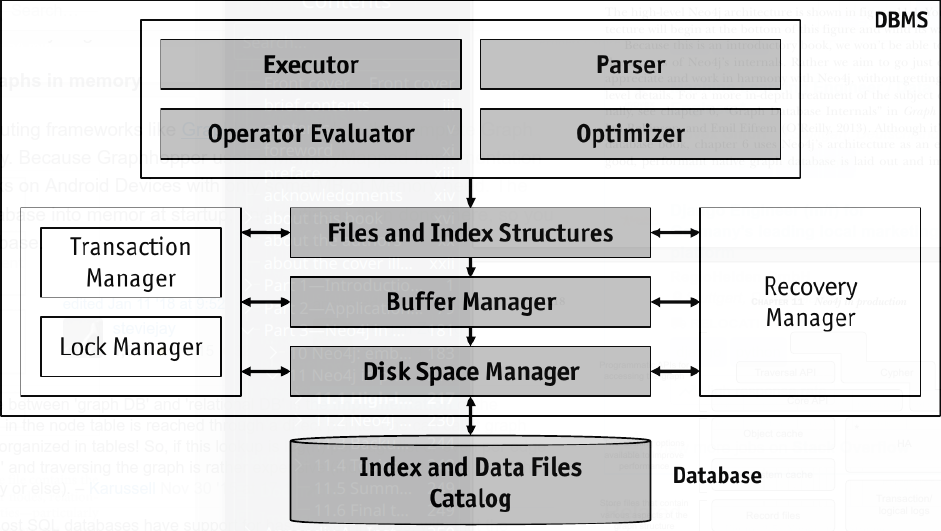
\includegraphics[keepaspectratio,width=0.7\textwidth]{img/00_intro/RDBMS.png}
        \end{center}
        \caption{The typical structure of a relational database management system.} %TODO citation
        \end{figure}

        Here The disk space manager, sometimes also called storage manager, handles de-/allocations, reads \& writes and provides the concept of a page: A disk block brought into memory. 
        For that it needs to keep track of free blocks in the allocated file. Optimally both a disk block and a page are of the same size. 
        One crucial task of a disk space manager is to store sequences of pages into continuous memory blocks in order to optimize data locality.
        Data locality has the upside, that one needs only one I/O operation to load multiple pages.
        To summarize the two most important objectives of a storage manager are to provide a locality-preserving mapping from pages to blocks based upon the information in the DBMS and to abstract physical storage to pages, taking care of allocation and access.
        
        A buffer manager is used to mediate between external storage and main memory. It maintains a designated pre-allocated area of main memory --- called the buffer pool --- to load, cache and evict pages into or from main memory.
        It's objective is to minimize the number of disk reads to be executed by caching, pre-fetching and the usage of suitable replacement policies. 
        It also needs to take care of allocating a certain fraction of pages to each transaction.

        \begin{figure}[htp]\label{dbms_memory}
            \begin{center}
            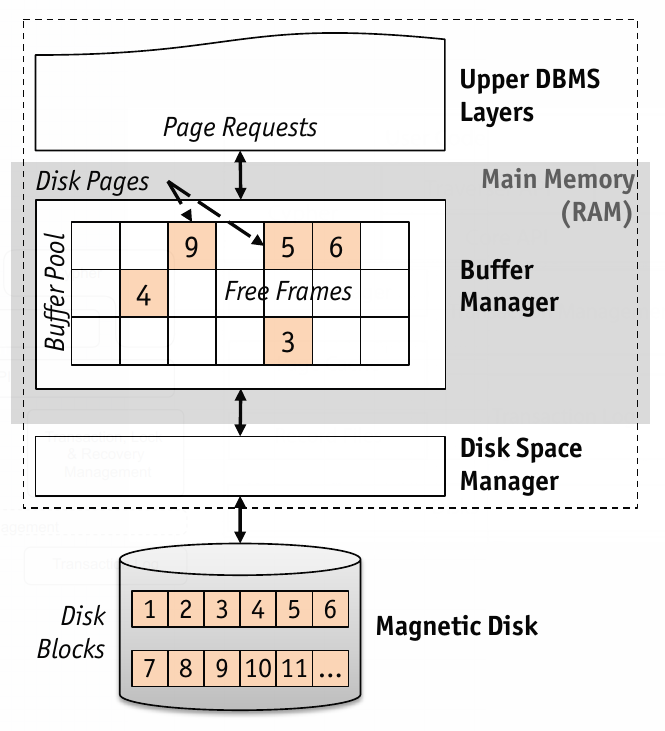
\includegraphics[keepaspectratio,height=0.4\textheight,width=0.5\textwidth]{img/00_intro/RDBMS_memory_view.png}
            \end{center}
            \caption{A visualization of the interaction of a database with memory.} %TODO citation
        \end{figure}

        The final memory and storage model relevant component of the  of a database management system is the file layout and possible index structures. 
        In order to store data a DBMS may either store one single or multiple files to maintain records. 

        A file may consist of a set of pages containing a set of slots. A slot stores one record with each record containing a set of fields. Further the database needs to keep track of free space in the file: A linked list or a directory must record free pages and some structure needs to keep track of the free slots either globally or per page. 
        Records may be of fixed or of variable size, depending on the types of their fields. 
        Records can be layout in row or column major order.
        That is one can store sequences of tuples or sequences of fields.
        The former is beneficial if a lot of update, insert or delete operations are committed to the database, while the latter optimizes the performance when scans and aggregations are the most typical queries to the system.
        Another option is to store the structure of the records along with pointers to the values of their fields in one files and the actual values in one or multiple separate files. 
        Also distinct types of tables can be stored in different files. 
        For example entities and relations can be stored in different files with references to each other, thus enabling the layout of these two to be specialized to their structure and usage in queries.

        Files may either organize their records in random order (heap file), sorted or using a hash function on one or more fields. 
        All of these approaches have upsides and downsides when it comes to scans, searches, insertions, deletions and updates. 

        To mitigate the effect that result from selecting one file organization or another, the concept of indexes have been introduced. 
        Indexes are auxiliary structures to speed up certain operations that depend on one field. 
        Indexes may be clustered or unclustered. 
        An index over field $F$ is called clustered if the underlying data file is sorted according to the values of $F$. 
        An unclustered index over field $G$ is one where the file is not sorted according to $G$. 
        In a similar way indexes can be sparse or dense. 
        A sparse index has less index entries than records, mostly one index entry per file. 
        This can of course only be done for clustered indexes as the sorting of the data file keeps the elements between index keys in order. 
        An index is dense if there is a one to one correspondence between records and index entries. 
        There are different variants of storing index entries which have again certain implications on the compactness of the index and the underlying design decisions.

        In another view of database management systems architectures, this boils down to the design decisions one has to make when implementing the storage layer and the access layer as shown in figure~\ref{dbms_arch_layers}.

        \begin{figure}[htp]\label{dbms_arch_layers}
        \begin{center}
        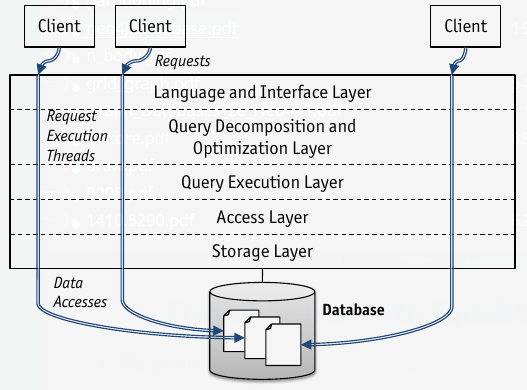
\includegraphics[keepaspectratio,width=0.6\textwidth]{img/00_intro/layered_RDBMS.png}
        \end{center}
        \caption{The architecture of a database management system from another point of view.} %TODO citation
        \end{figure}

        Here the storage layer is in close correspondence to the disk space manager in combination with the buffer manager, while the files and index structures provide the access layer.

        All these considerations make choosing different file splits, layouts, orderings, addressing schemes, management structures, de-/allocation schemes and indexes a complex set of dependent choices. 
        These depend mainly on the structure of the data to be stored and the queries to be run.
        
        % TODO Elaborate on get nodes, get relationships and expand


    \subsection{The Property Graph Model}\label{\positionnumber}
        The property graph model is a widely adopted data model to represent graphs in databases.
        It is not only able to represent the structure of directed or undirected, weighted or unweighted, but also of typed graphs carrying additional information.
    
        A \textbf{Property Graph} is a 9-Tuple $G = (V, E, \lambda, P, T, L, f_P, f_T, f_L)$ with 
        \begin{itemize}
            \item $V$ the set of vertices.
            \item $E$ the set of edges.
            \item $\lambda: (V \times V) \rightarrow E$ a function assigning a pair of nodes to an edge.
            \item $L$ a set of strings used as labels.
            \item $P$ a set of key-value pairs called properties.
            \item $T$ a set of strings used as relationship types.
            \item $f_P: V \cup E \rightarrow 2^P$ a function that assigns a set of properties to a node or relationship.
            \item $f_T: E \rightarrow T$ a function that assigns a type to  a relationship.
            \item  $f_L: V \rightarrow 2^L$ a function that assigns a node a set of labels.
        \end{itemize} 
        \smallskip
        The property graph model reflects a directed, node-labeled and relationship-typed multigraph $G$, where each node and relationship can hold a set of key-value pairs~\cite{angles2018property}. \\
        In a graph the edges are normally defined as $E \subseteq (V \times V)$, but in the property graph model edges have sets of properties and a type, which makes them records on their own. 
        This means they either need to be addressed explicitly or one needs to store all information, including the properties, consecutively. 
        The latter approach has the downside, that when the type or a property contain a variable length string, the relationships have to be variable lenght records. 
        This would cause the lookup of a relationship's property to be not only indirected via a node index, but also requires an additional mechanism to be able to tell the beginning and length of the record. \\
        An illustration of this model is shown in \fullref{fig:propertygraph}\fig{img/property_graph_elements.jpg}{propertygraph}{A visualization of the property graph model}{1}.
        Neo4j is a graph database employing the property graph model~\cite{neo4j_book}, which is used in the evaluation part of this thesis.
    
    \subsection{Example: Neo4J}\label{\positionnumber}
        When restricting to graph structures where nodes and relationships are allowed to have properties and labels and types respectively, this allows one to narrow down some of the design decisions.
        In particular the example of a popular graph native database --- Neo4J --- is what we discuss in this subsection.

        To get an overview of the architecture let us consider figure~\ref{N4J_HLA_Emil}. 

        \begin{figure}[htp]\label{N4J_HLA_Emil}
        \begin{center}
        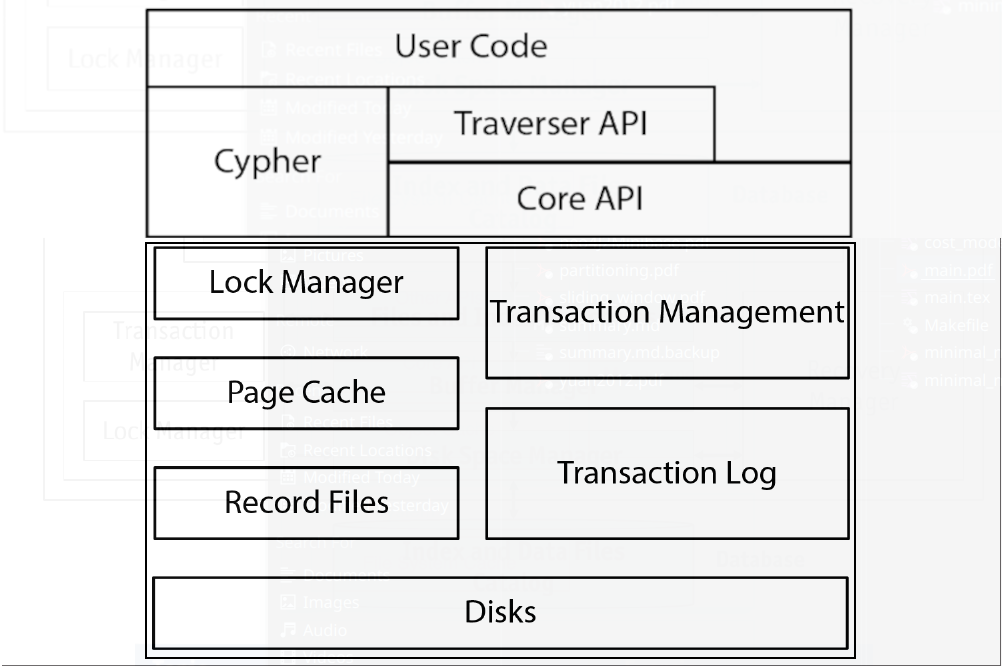
\includegraphics[keepaspectratio,width=0.6\textwidth]{img/00_intro/N4J_HLA_Emil.png}
        \end{center}
        \caption{The high level architecture of Neo4J according to Emil Efrim, the co-founder of Neo technologies.} %TODO citation
        \end{figure}

        Here we can see that the previous schema is not exactly straight forward to apply, mainly due to a lack of concise documentation.
        The diagram was taken from the only publication that elaborates on the internals of Neo4J aside from the code of course.
        
        \begin{figure}[htp]\label{N4J_Storage}
        \begin{center}
        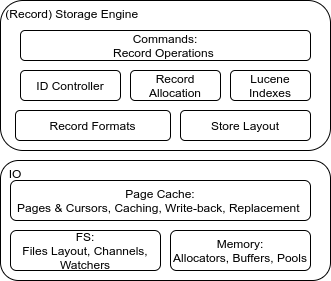
\includegraphics[keepaspectratio,width=0.5\textwidth,height=0.3\textheight]{img/00_intro/N4J_Storage.png}
        \end{center}
        \caption{A visualization of the broad the storage and memory organization of Neo4J.} %TODO citation
        \end{figure}
        
        Here The storage manager makes mostly use of the Java NIO package with some additional usage of operating system native calls to allocate memory for the page cache and network buffers. 
        A more detailed view on the high level architecture of the disk space and buffer manager and the files and index structures was deduced by the author from the source code and the non-public JavaDocs.
        This is shown in figure~\ref{N4J_Storage}.
        
      \begin{figure}[htp]\label{N4J_memory_view}
        \begin{center}
        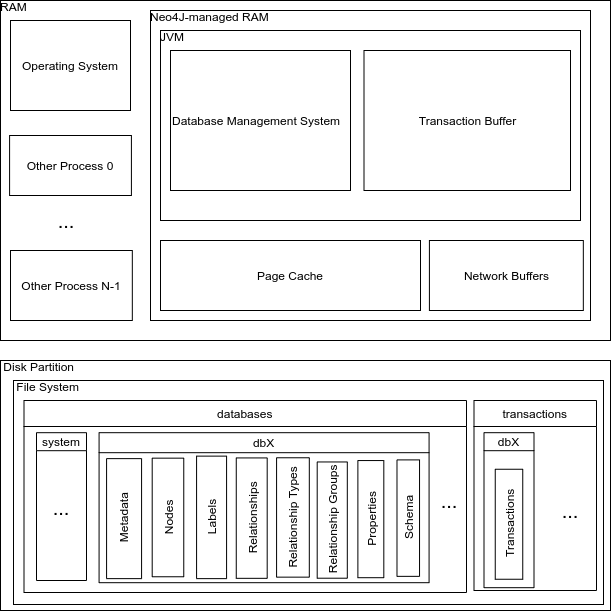
\includegraphics[keepaspectratio,width=0.6\textwidth]{img/00_intro/N4J_memory_view.png}
        \end{center}
        \caption{A sketch of how Neo4J occupies memory.} %TODO citation
        \end{figure}
        
        The overall memory and storage state of a Neo4J instance and its environment may thus be visualized like this figure~\ref{N4J_memory_view}.

        \subsubsection{IO \& File Layout}\label{files_sec}
        The files that Neo4J uses to store data are categorizable into 5 classes based upon the records they contain:
        \begin{itemize}
            \item Node-related files: These files start with the prefixes \mintinline{bash}{neostore.nodestore*} and \mintinline{bash}{neostore.label*}. 
                The contents of these files contain the node structure and labels. 
            \item Relationship-related files: The prefix \mintinline{bash}{neostore.relationship*} is used for all files containing records related to the graph's relationship structure, types and possibly groups.
            \item Property-related files: Containing the properties of both nodes and relationship, this is the part that is least structured and rather unspecialized with respect to graphs.
            \item Schema: Files starting with \mintinline{bash}{neostore.schemastore*} contain information about the schema of the graph or rather the schematic information on the node, relationship and property labels, types and constraints.
            \item Metadata: Files only starting with \mintinline{bash}{neostore} and none of the above prefixes contain meta information about the graph.
            \item Finally, a lock file.
        \end{itemize}
        
        \begin{figure}[htp]\label{files}
            \begin{center}
                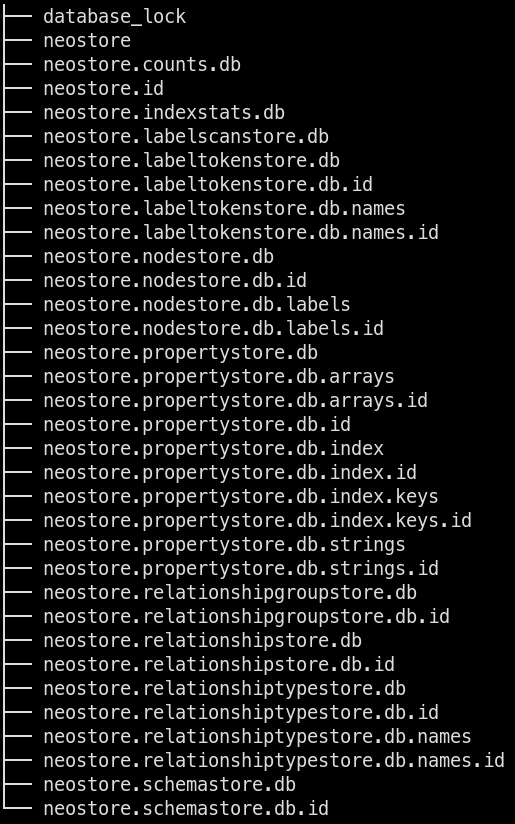
\includegraphics[keepaspectratio,height=0.4\textheight,width=0.5\textwidth]{img/03_record/files.png}
            \end{center}
            \caption{A visualization of the files layout of Neo4j.} %TODO citation
        \end{figure}

        Most importantly the files ending with \mintinline{bash}{.db} contain all fixed size records representing the structure of the graph and small amounts of data.
        Files ending with \mintinline{bash}{.id} are used for record allocation and contain unused IDs. 
        Files having one of the suffixes \mintinline{bash}{names}, \mintinline{bash}{arrays} and \mintinline{bash}{strings} are so called dynamic stores and contain dynamic sized records. 
        A dynamic store is always started with a header block containing extra information and the offset to the first block in the store files. 
        Files ending with \mintinline{bash}{.index} contain indexes either generated by Neo4J (e.g.\ the keys of properties are referenced like this to avoid storing key names multiple times) or by the Apache Lucene indexing library.
        
        \subsubsection{Record Structures}
            \paragraph{Address Translation}
                Neo4j defines the following constants as the size of the addresses used.
                \begin{figure}[htp]\label{addrsize}
                    \adjustbox{varwidth=\textwidth, scale=0.9}{%
                        \inputminted{Java}{code/MaxIdLength.java}
                    }
                \end{figure}
                These are represented by the datatype \mintinline{java}{long} when loaded into main memory. 
                On disk these values are stored as 32-bit \mintinline{java}{Integer}s with additional modifiers, that is the highest bits that do not fit into an int are stored to fields with additional space.
                
                For example the in-use bit consumes one byte of memory and the additional 7 bytes are used to stroe the highest bits that do not fit into an integer of another field.
                
                Finally the base and the modifer are aggregated into a long by shifting both appropriately, casting them to longs and applying the logical or \mintinline{java}{|} operation.
                
                Thus when refering to high bits and ID below, high bits do always mean the remainer of the bits that did not fit into the field that is said to be holding the ID\@.
                The latter is actually only holding the lowest 32 bits of an ID/address. The \textit{actual ID} is always high bits and ID field, shifted appropriately and connected using the logical or operator.
                
            \paragraph{Nodes}
                The record format of nodes consist of a 15 byte structure.
                The IDs of nodes are stored implicitly as their address.
                If a node has ID 100 we know that its record starts at offset $15 \text{ Bytes} \cdot 100 = 1500$ from the beginning of the file.
                The struct of a record looks like this:
                \begin{enumerate}
                    \item Byte 1: The first byte contains one bit for the in-use flag. 
                        The additional 7 bits are used to store the 3 highest bits of the relationship ID and the 4 highest bits of a property ID\@.
                    \item Bytes 2 --- 5: The next 4 Bytes represent the ID of the first relationship in the linked list containing the relationships of the considered node.
                    \item Bytes 6 --- 9: Again 4 bytes encode the ID to the first property of the node.
                    \item Bytes 10 --- 14: This 5 byte section points to the labels of this node.
                    \item Byte 15: The last byte stores if the node is dense, i.e.\ one node has an aweful lot of relationships and is treated a bit differently.
                        That is a relationships are stored by type and direction for this node into groups, see~\ref{rel_group}.
                \end{enumerate}
            
                \begin{figure}[htp]\label{node_record}
                    \begin{center}
                        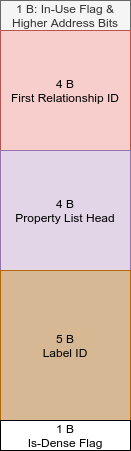
\includegraphics[keepaspectratio,height=0.4\textheight,width=0.5\textwidth]{img/03_record/node/node_record.png}
                    \end{center}
                    \caption{A visualization of the record structure of a node.} %TODO citation
                \end{figure}
                
                To summarize: The records on disk are stored as in the enumeration above. 
                In the database all IDs get mapped to longs and their respective space is larger than the space representable by 35 bit --- what is perfectly fine.
            
                \begin{figure}[htp]\label{node_first_byte}
                    \begin{center}
                        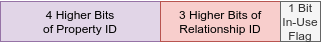
\includegraphics[keepaspectratio,height=0.4\textheight,width=0.5\textwidth]{img/03_record/node/node_first_byte.png}
                    \end{center}
                    \caption{A visualization of the information stored in the first byte of a node record.} %TODO citation
                \end{figure}
            
                On disk 4 byte integers are used to store the 32 lowest bits of the respective addresses and the higher bits are stored in the first byte that also carries the in-use bit.
            
            \paragraph{Node Labels}
                Each node label record consists of an in use bit and a name ID, which in turn points to an entry in a seperate file storing label names as dynamic records (see~\ref{dynamic}), storing the label names.
                This is done in order to assure that the records are of fixed length.
                \begin{enumerate}
                    \item Byte 1: In-use flag
                    \item Bytes 2 --- 5: Pointer to the label string entry
                \end{enumerate}
                
                \begin{figure}[htp]\label{label_record}
                    \begin{center}
                        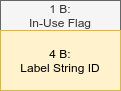
\includegraphics[keepaspectratio,height=0.2\textheight,width=0.2\textwidth]{img/03_record/node/label_record.png}
                    \end{center}
                    \caption{A visualization of the structure of a label record.} %TODO citation
                \end{figure}
                
                
            
            \paragraph{Relationships}
                \begin{figure}[htp]\label{rel_record}
                    \begin{center}
                        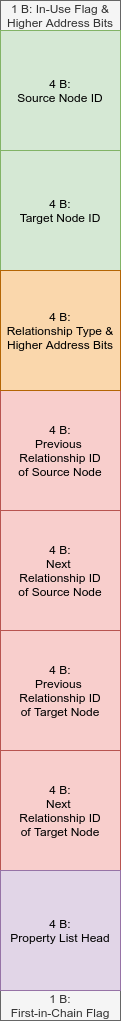
\includegraphics[keepaspectratio,height=0.9\textheight,width=0.5\textwidth]{img/03_record/relationship/relationship_record.png}
                    \end{center}
                    \caption{A visualization of the record structure of a relationship in Neo4J.} %TODO citation
                \end{figure}
                
                Relationship records are stored with implicit IDs too. 
                Their fixed size records contain 34 bytes.
                Besides an in-use flag and the node IDs that are connected, and the relationship type, the record also contains two doubly linked list: One for the relationships of the first node and one for the relationship of the second node.
                Finally a link to the head of the properties linked list of this relationship and a marker if this relationship is the first element in the relationships linked list of one of the nodes.
                \newpage
                
                \begin{enumerate}
                    \item Byte 1: In-use bit, first node high order bits (3 bits), first property high order bits (4 bits)
                    \item Bytes 2 --- 5: first node ID 
                    \item Bytes 6 --- 9: second node ID 
                    \item Bytes 10 --- 13: relationship type (16 bit), second node high order bits (3 bits), relationship previous and next ID higher bits for first and second node ($4 \cdot 3 = 12$ bits), one unused bit.
                    \item Bytes 14 --- 17: previous relationship ID for first node
                    \item Bytes 18 --- 21: next relationship ID for first node
                    \item Bytes 22 --- 25: previous relationship ID for second node
                    \item Bytes 26 --- 29: next relationship ID for second node
                    \item Bytes 30 --- 33: link to the first property of the relationship
                    \item Bytes 34: A marker if this relation is the first element in the relationship linked list of one of the nodes stored in the lowest two bits of the byte. 
                        The other 6 bits are unused.
                \end{enumerate}


                \begin{figure}[htp]\label{rel_first_byte}
                    \begin{center}
                        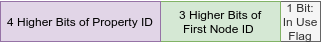
\includegraphics[keepaspectratio,width=\textwidth]{img/03_record/relationship/relationship_first_byte.png}
                    \end{center}
                    \caption{A visualization of how information is stored in the first byte of a relationship record.} %TODO citation
                \end{figure}

                \begin{figure}[htp]\label{rel_type_bytes}
                    \begin{center}
                        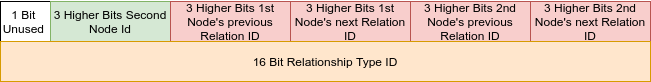
\includegraphics[keepaspectratio,width=\textwidth]{img/03_record/relationship/relationship_type_bytes.png}
                    \end{center}
                    \caption{The structure of the bytes that are used to store the type of a relationship and high bits of a node and a relationship IDs.} %TODO citation
                \end{figure}
            

            \paragraph{Relationship Types}
                Similarly to the node labels, the relationship type records posses an in-use flag and a type ID that points to a record in a file containing strings in the dynamic record format.
                \begin{enumerate}
                    \item Byte 1: In-use flag
                    \item Bytes 2 --- 5: Pointer to the type string entry
                \end{enumerate}
            
                \begin{figure}[htp]\label{rel_type_record}
                    \begin{center}
                        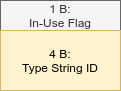
\includegraphics[keepaspectratio,height=0.2\textheight,width=0.2\textwidth]{img/03_record/relationship/rel_type_record.png}
                    \end{center}
                    \caption{A visualization of the record structure of a relationship type.} %TODO citation
                \end{figure}
                
           
           All further record structures like properties, arrays and strings are omitted for the sake of succintness.
        
        \subsubsection{Caching \& Indexes} 
        
        \subsubsection{Queries \& Transactions}
            
            
    \subsection{Locality}\label{\positionnumber}
        
        \subsubsection{Metrics}
    



